% Preamble
\documentclass[11pt]{article}

% Packages
\usepackage{amsmath}
\usepackage{graphicx}
\usepackage{hyperref}
\usepackage[all]{hypcap}
\usepackage{polski}
\usepackage{xcolor}
\usepackage[a4paper, total={6in, 8in}]{geometry}
\usepackage{multirow}

\definecolor{new_orange}{HTML}{ff5500}

\hypersetup{
    colorlinks=true,
    linkcolor=new_orange,
    filecolor=magenta,
    urlcolor=blue,
    citecolor=new_orange
}

% Graphics directory
\graphicspath{ {./figures/} }

% Title and authors

\title{\textbf{Analiza danych ankietowych - sprawozdanie II}}
\author{Aleksandra Miedzińska, Nikodem Drelak}

% Document
\begin{document}

    \maketitle
{
  \hypersetup{linkcolor=black} % Tymczasowo zmień kolor na czarny
  \tableofcontents
}


    \section{Wstęp}\label{sec:wstep}

    cos tam o rysunku~\ref{fig:fig1})

    \begin{figure}[hp]
        \centering
        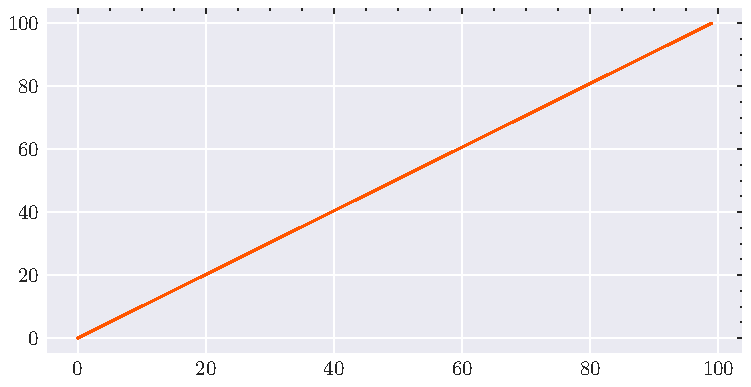
\includegraphics[width=1\textwidth]{figure1}
        \caption{Przykladowy rysunek}
        \label{fig:fig1}
    \end{figure}

\phantomsection
\addcontentsline{toc}{section}{Literatura}
\bibliographystyle{unsrt}
\bibliography{bibliografia}

\end{document}